\renewcommand{\inputfile}{\version\ - Predrag edited 2009-02-28 symODEs}
% section: Symmetries of dynamical systems
% $Author$ $Date$

% For more
% details the reader is referred to the monographs of Golubitsky and
% Stewart\rf{}, Chossat and Lauterbach\rf{}, Hoyle\rf{} and Olver\rf{}.


We consider a system of \ode s of the form
\beq
	\dot{x} = \vf(x,\lambda)
	\label{eq:difeq}
\eeq
where $\vf: \Rls{n}\times\Rls{r} \rightarrow \Rls{n}$ a $C^\infty$ mapping. When
not important we will suppress the $r$-dimensional vector of parameters
$\lambda$ in the notation.

Any compact Lie group acting on $\Rls{n}$ can be identified
with a subgroup of $\On{n}$, \cf\ for example \refref{golubII}
for a sketch of the proof. Therefore, without loss of generality
we will concentrate on subgroups $\Gamma\subseteq\On{n}$ in the following.
    \PC{Aren't you supposed to define Lie group, algebra in this chapter?
        I do not like ${\tt Lg} = \mathfrak{g}$ as the notation for
        the Lie algebra generator - it confuses it with the finite
        action group element $g$. Something like
        ${\tt Lg} = \mathfrak{a}$ would make more sense. Are you
        following some reputable literature with this notation?{\bf ES:} Changed
	it, I also didn't like it and no, I wasn't following any text.
	I thought I could get away without defining them, at least not having
	to say what a group is. If I just say group generator and drop the term
	algebra, wouldn't it be more familiar to physicists?}


\begin{definition}
\label{def:symmetry}
\index{symmetry}
We call a group element $\gamma\in\On{n}$ a symmetry of \refeq{eq:difeq} if for every solution
$x(t)$, $\gamma x(t)$ is also a solution.
\end{definition}\ES{Refer to point vs contact symmetries?}

The question now arises on how to check for symmetries of \refeq{eq:difeq} since
we generally do not have knowledge of the set of solutions\ES{Rather naively put.}. Let $x(t)$ be a solution
of \ref{eq:difeq}. Then by \refDef{def:symmetry} $y(t)=\gamma x(t)$ is another solution
and therefore satisfies \refeq{eq:difeq}:
\[
 \dot{y}(t)=\vf{\PCedit{(y(t))}}=\vf(\gamma x(t))\,.
\]
On the other hand
\[
 \dot{y}(t)=\gamma \dot{x} = \gamma \vf(x(t))\,,
\]
for any solution $x(t)$. Since solutions exist for any $x\in\Rls{n}$ we are led to the following
condition for $\gamma$ to be a symmetry of \refeq{eq:difeq}:
\beq
	\vf(\gamma x) =\gamma \vf(x)
	\label{eq:equiv}
\eeq
for all $x\in\Rls{n}$. We say that $\vf$ \emph{commutes} with $\gamma$ or that $\vf$ is $\gamma$-\emph{equivariant}.
When $\vf$ commutes with all $\gamma\in\Gamma$ we say that $\vf$ is $\Gamma$-equivariant\index{equivariant}.
In physics literature the term $invariant$ is most commonly used, mostly because in Hamiltonian systems
symmetry is manifested as invariance of the Hamiltonian under the symmetry operation.
% When $f$ is $\gamma$-equivariant
% the \ode~ \ref{eq:difeq} remains invariant under the action of $\gamma$.
Clearly the finite time flow $\flow{t}{\gamma x_o}$ through $\gamma x_o$
satisfies the equivariance condition $\flow{t}{\gamma x_o}=\gamma \flow{t}{x_o}$ from
definition of symmetry and uniqueness of solutions.

\begin{example}
\index{Lorenz flow!symmetry}
The vector field in Lorenz equations \refeq{Lorenz} is equivariant under the group
$\Zn{2}\cong\Dn{1}$ acting on \Rls{3}\ by
\[
	\Rot{\pi}(x,y,z) = (-x,-y,z)\,.
\]
Note that this transformation can be considered either as rotation by $\pi$ around the $z$ axis (hence the
group \Zn{2}) or as reflection about the origin in a plane perpendicular to the $z$-axis (hence the group \Dn{1}.)
\end{example}

\begin{example}
\index{Complex Lorenz flow!symmetry}
The vector field in \CLe\ \refeq{eq:CLe} is equivariant under the group \SOn{2} acting on $\Rls{5}\cong \Clx{2}\times \Rls{}$
by
\beq
 \Rot{\theta} (x,y,z) = (e^{i\theta} x, e^{i\theta} y, z)\,,\ \ \  \theta\in[0,2\pi)\,.
 \label{eq:RotCLe}
\eeq
\end{example}

\begin{example}
\index{Armbruster-Guckenheimer-Holmes flow!symmetry}Finally, the symmetry group of the \AGHe
\begin{subequations}\label{eq:AGH}
\begin{align}
  \dot{z}_1 &=\bar{z}_1 z_2
              + z_1\left(\mu_1+ e_{11}|z_1|^2+e_{12}|z_2|^2\right) \\
  \dot{z}_2 &=\pm z_1^2
              + z_2\left(\mu_2+ e_{21}|z_1|^2+e_{22}|z_2|^2\right)
\end{align}
\end{subequations}
is \On{2} acting by
\begin{subequations}
\begin{align}
  \Rot{\theta}(z_1,z_2) &= (e^{i\theta} z_1, e^{i 2\theta} z_2)\,,\ \ \  \theta\in[0,2\pi)\,,\\
  \Refl(z_1,z_2) &= (\conj{z}_1,\conj{z}_2)\,.
\end{align}
\end{subequations}
\end{example}

\subsection{\Statesp\ stratification}
\label{sec:strata}

In order to understand the implications of equivariance for the solutions
of \refeq{eq:difeq} we first have to examine the way a compact
Lie group acts on \Rls{n}.

\index{group orbit} The \emph{group orbit} of $x\in\Rls{n}$ is the set
\beq
	\Gamma x = \{\gamma x: \gamma\in\Gamma\}\,.
\eeq


% \begin{definition}
% \label{def:stab}
% \index{isotropy subgroup}\index{stabilizer}
%  The isotropy subgroup or stabilizer of a subset $S\subset \Manif$ is the set
%  \beq
%   	\stab{S}=\{\gamma\in\Gamma:\gamma S=S\}\,.
%  \eeq
% \end{definition}
% Thus the isotropy subgroup describes the symmetries of a set $S$. Note that by
% \refDef{def:stab} the isotropy subgroup is the largest subgroup (in the
% sense of set inclusion, \cf \refeq{eq:Gorder}) that leaves $S$ fixed.
% % Most often we will restrict our attention to the isotropy subgroup of a single point $x\in\Manif$.

% ES commented out definition of isotropy subgroup of a point
\begin{definition}
\label{def:stab}
\index{isotropy subgroup}\index{stabilizer}
The isotropy subgroup or stabilizer of $x\in\Manif$ as
\beq
	\stab{x}=\{\gamma\in\Gamma:\gamma x=x\}\,.
\eeq
\end{definition}
Thus the isotropy subgroup describes the symmetries of a point $x$. Note that by
\refDef{def:stab} the isotropy subgroup is the largest subgroup (in the
sense of set inclusion, \cf \refeq{eq:Gorder}) that leaves $x$ fixed.
% PC commented this out: The following lemma
% relates the isotropy subgroups of points on the same group orbit.

% \begin{definition}
% \label{def:GlobStab}
% \index{isotropy subgroup!global}
%  The global isotropy subgroup of a subset $S\subset \Manif$ is the set
%  \[
%   	\globstab{S}=\bigcap_{x\in S} \stab{x} = \{\gamma\in\Gamma:\gamma x=x\,,\ \forall x\in S\}\,.
%  \]
% \end{definition}


\begin{lemma}
\label{lem:stabGorbit}
Points on the same group orbit of $\Gamma$ have conjugate isotropy subgroups:
\beq
	\stab{\gamma x}=\gamma \stab{x} \gamma^{-1}\,.
\eeq
\end{lemma}
(See \refref{golubII} for the proof.)
%
% \refLem{lem:stabGorbit} implies that
Thus we can characterize a group orbit by its \emph{type}, defined
as the conjugacy class of its isotropy subgroups.

\begin{proposition}
 \label{pro:dimOrb}
 Let $\Gamma$ be a compact Lie group acting on \Rls{n}. Then
 \begin{enumerate}
  \item If $\Gamma$ is finite then $|\Gamma|=|\stab{x}||\Gamma x|$.
  \item If $\Gamma$ is continuous then $\dim \Gamma = \dim \stab{x}+\dim \Gamma x$.
 \end{enumerate}
\end{proposition}
The proof can be found in \refref{golubII}. We note that
% PC commented out: a useful relation from the proof:
$\dim\Gamma x =\dim(\Gamma/\stab{x})$, where the \emph{coset space} of
a subgroup $\Sigma$  of $\Gamma$ is defined as
$\Gamma/\Sigma=\{\gamma\Sigma|\gamma\in\Gamma\}$.
Also recall that the (left) \emph{cosets} of $\Sigma$ in $\Gamma$ are the sets
$\gamma\Sigma=\{\gamma\sigma|\sigma\in\Sigma\}$.


\index{stratum}
Therefore, when $\Gamma$ is continuous each group orbit is a smooth compact manifold of dimension
$\dim \Gamma x=\dim \Gamma-\dim \stab{x}$. The union of orbits of the same type is called a \emph{stratum}
and is itself a smooth manifold. Thus \Rls{n} is stratified by the action of $\Gamma$ into
a disjoint union of strata $\Str{i}$ which are in an $1-1$ correspondence to the group orbit types (\cf~\refref{ChossLaut00} for proof.)
Note that in general the strata do not have the same dimension. There exists a unique stratum \Str{0} of maximal
dimension that is called \emph{principal stratum}\rf{gatermannHab}. The principal stratum is open, dense
and if $\Gamma$ is connected then \Str{0} is also connected\rf{ChossLaut00}.

\begin{definition}
 \label{def:fixedsp}
 \index{fixed-point subspace} Let $\Sigma$ be a subgroup of $\Gamma$ acting on \Rls{n}. The \fixedsp\ of $\Sigma$,
 denoted by $Fix(\Sigma)$, is the subspace of \Rls{n} containing all fixed points of $\Sigma$:
\[
	Fix(\Sigma)=\{x\in\Rls{n}\ |\ \sigma x = x\,,\ \forall \sigma\in\Sigma\}\,.
\]
\end{definition}

\Fixedsp s are invariant under equivariant dynamics. The following theorem applies:

\begin{theorem}
 Let $f:\Rls{n}\rightarrow\Rls{n}$ be $\Gamma$-equivariant and let $\Sigma$ be a subgroup of $\Gamma$. Then
\[
 f\left(Fix(\Sigma)\right)\subseteq Fix(\Sigma)\,.
\]
\end{theorem}\ES{write the proof}

This leads to:
\begin{proposition}
 Let $x(t)$ be a solution trajectory of an equivariant ODE. Then $\Sigma_{x(t)}=\Sigma_{x(0)}$ for all $t$.
\label{pro:gfInv}
\end{proposition}\ES{write the proof}

Let $A(x)=\frac{\partial\vf(x)}{\partial x}$ and use the chain rule:
\beq
	A(\gamma x) \gamma = \gamma A(x)\,, \qquad \gamma\in\Gamma\,.
	\label{eq:LrzGroupOrb}
\eeq
Then, for $\gamma\in\stab{x}$ we have
\beq
	A(x) \gamma = \gamma A(x)\,, \qquad \gamma\in\stab{x}.
	\label{eq:LrzCommut}
\eeq
\ie the stability matrix at $x$ commutes with $\stab{x}$.\ES{Discuss restriction in form of $A(x)$,
eigenvectors.}

We can define a partial ordering $\preceq$ on conjugacy classes of subgroups of $\Gamma$. Let $H=\{H_i\}$ and $K=\{K_j\}$
be two such conjugacy classes. Then
\beq
	H\preceq K \Leftrightarrow H_i\subseteq K_j
	\label{eq:Gorder}
\eeq
for some representatives $H_i,\,K_j$. We refer to the partially ordered set that results from this ordering as the \emph{subgroup lattice}.

\begin{definition}
 The isotropy lattice of $\Gamma$ is the set of all conjugacy classes of isotropy subgroups
 partially ordered by $\preceq$.
\end{definition}
    \ES{
I copy Golubitsky and Stewart's definition of isotropy lattice and partial ordering (but not of subgroup lattice)
here because I am somewhat confused. Are the conjugacy classes of subgroups distinct
from the classes defined by conjugate elements of the group?
For instance in the example of \Dn{3} below, $\Ztwo(\Refl)$, $\Ztwo(\Refl \Drot)$
and $\Ztwo(\Refl \Drot^2)$ are conjugate subgroups. My interpretation is that we call this
a conjugacy class of isotropy subgroups.
On the other hand, \Dn{3} is partitioned in three classes: $\{e\},\{\Refl,\Refl\Drot,\Refl\Drot^2\}$
and $\{\Drot,\Drot^2\}$ which of course are not subgroups, except for $\{e\}$.
    }
\ES{We know that we can consider vector spaces as groups under addition and then subspaces
are subgroups. How is the isotropy lattice connected to this picture?}

\begin{definition}
 Let $\Sigma$ be a subgroup of $\Gamma$. The normalizer of $\Sigma$ in $\Gamma$ is
 $\Nlz{\Sigma}=\{\gamma\in\Gamma\, |\, \gamma\Sigma\gamma^{-1}=\Sigma\}$.
\end{definition}

\begin{lemma}
  The largest subgroup of $\Gamma$ that acts\ES{this means that group orbits under \Nlz{\Sigma} are on \Fix{\Sigma}} in \Fix{\Sigma} is \Nlz{\Sigma}.
  \label{lem:NlzActs}
\end{lemma}
For proof \cf \refref{ChossLaut00}.



\begin{example} % Subgroups of \Dn{3}
Consider \Dn{3}, the symmetry group of the equilateral triangle
\reffig{fig:D3triangle}, acting on $\Rls{2}\cong\Clx{}$ by
\begin{subequations}\label{eq:D3onR2}
\begin{align}	
  \Drot z &= e^{i\frac{2\pi}{3}} z\,,\\
  \Refl z  &= \conj{z}\,.
 \end{align}
\end{subequations}

%%%%%%%%%%%%%%%%%%%%%%%%%%%%%%%%%%%%%%%%%%%%%%%%%%%%%%%%%%%%%%%%
\begin{figure}
    % \vspace*{-5pt}
\begin{center}
		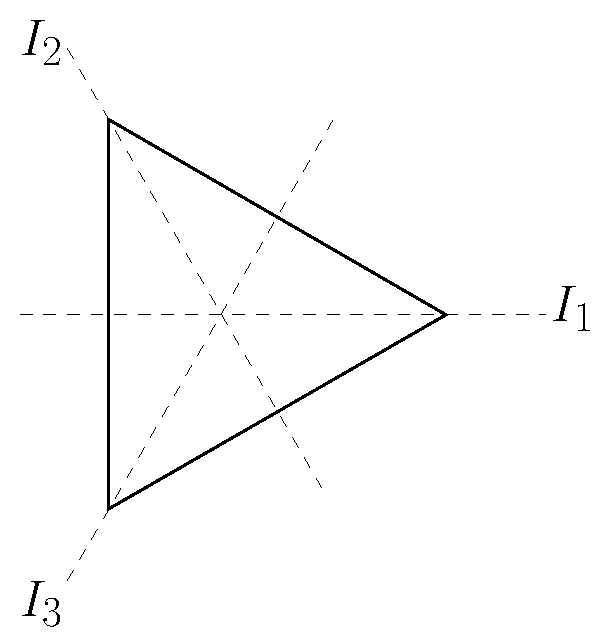
\includegraphics[width=0.25\textwidth]{../figs/D3triangle}
\end{center}
\caption[\Dn{3} symmetry illustration]{
    {\small
    \Dn{3} leaves the equilateral triangle setwise fixed.
    The reflection symmetry axes have been denoted $I_i$.}}
\label{fig:D3triangle}
    \vspace*{-5pt}
\end{figure}
%%%%%%%%%%%%%%%%%%%%%%%%%%%%%%%%%%%%%%%%%%%%%%%%%%%%%%%%%%%%%%%%%

There are, up to conjugacy, three subgroups: $\Idg=\{e\}$, $\Ztwo(\Refl)$,
which is isomorphic\ES{or say conjugate?} to the subgroups generated
by $\Refl\Drot$ and by $\Refl\Drot^2$, and $\Cn{3}=\{e,\Drot,\Drot^2\}$.
The subgroup lattice is shown in \reffigpart{fig:D3lattice}{a}.
There are three classes, each corresponding to
a distinct geometrical operation: $\{e\},\{\Refl,\Refl\Drot,\Refl\Drot^2\}$
and $\{\Drot,\Drot^2\}$.


\end{example}


\begin{example}  % Isotropy subgroups of \Dn{3}
We now examine how the vertex $A$ of the triangle transforms
under the action of \Dn{3}. Under $\Drot$ and $\Drot^2$ it is
mapped to the vertices $B$ and $C$, respectively.
Thus all vertices belong to the same group orbit and have
conjugate isotropy subgroups, from \refLem{lem:stabGorbit}.
Under $\Refl$ vertex $A$ remains fixed. Thus the isotropy
subgroup of point $A$ is $\stab{A}=\Ztwo(\Refl)$. By
\refLem{lem:stabGorbit} we have $\stab{B}=\Drot\,
\Ztwo(\Refl)\, \Drot^{-1} = \Ztwo(\Refl\Drot)$
and
    \PCedit{
$\stab{C}=\Drot^{-1}\, \Ztwo(\Refl)\, \Drot =
\Ztwo(\Refl\Drot^2)$.
    }
Next, note that $\Ztwo(\Refl)$ fixes
any point on the symmetry axis $I_1$, while $\Drot$ and
$\Drot^2$ map it to $I_2$ and $I_3$, respectively. The origin
is the only point fixed by any group operation, \ie~has
isotropy subgroup $\Dn{3}$. Finally, any point that is not on
one of the symmetry axes $I_1,\ I_2,\ I_3$ has trivial isotropy
subgroup. Thus we arrive to the following conclusions:

The isotropy subgroups are: $\stab{\{0\}}=\Dn{3}$,
$\stab{I_1^*}=\Ztwo(\Refl)\simeq\stab{I_2^*}\simeq\stab{I_3^*}$,
$\stab{\Rls{2}\backslash\{\cup I_i\}}=\Idg$, where $I_i^*=I_i\backslash\{0\}$. The fixed point
subspaces of \Dn{3}, $\Ztwo(\Refl)$, $\Ztwo(\Refl\Drot)$ and
$\Ztwo(\Refl\Drot^2)$ are the origin, $I_1$, $I_2$ and $I_3$,
respectively. The fixed point subspace of \Cn{3} is the origin
but, since \Cn{3} is a proper subgroup of \Dn{3}, it
does not qualify as isotropy subgroup of the origin
(\cf~\refDef{def:stab}.) Thus \Cn{3} is not in the isotropy
lattice of \Dn{3} acting on \Rls{2},
\cf~\reffigpart{fig:D3lattice}{b}.
    \PC{something is screwy with the \pCf\ analysis - there
        we keep \Cn{3}, I think...}

%%%%%%%%%%%%%%%%%%%%%%%%%%%%%%%%%%%%%%%%%%%%%%%%%%%%%%%%%%%%%%%%
\begin{figure}
    % \vspace*{-5pt}
\begin{center}
  (\textit{a})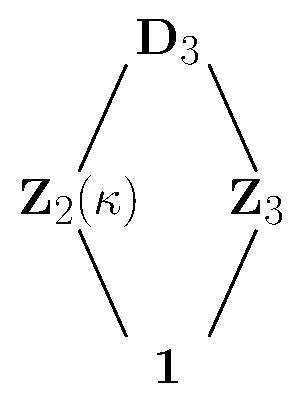
\includegraphics[height=0.15\textheight]{../figs/D3lattice}
~~~~(\textit{b})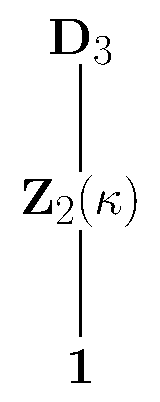
\includegraphics[height=0.15\textheight]{../figs/D3stablattice}
\end{center}
\caption[\Dn{3} lattices]{
    {\small
    (a) \Dn{3} subgroup lattice, (b) \Dn{3} isotropy lattice}}
\label{fig:D3lattice}
    \vspace*{-5pt}
\end{figure}
%%%%%%%%%%%%%%%%%%%%%%%%%%%%%%%%%%%%%%%%%%%%%%%%%%%%%%%%%%%%%%%%%

There are three strata in correspondence with the orbit types (and with isotropy subgroups): the origin (type \Dn{3}),
$\{\cup I_i^*\}$ (type $\Ztwo(\Refl)$), and the principal stratum $\Rls{2}\backslash\{\cup I_i\}$ (type $\Idg$).

If we now consider a two dimensional system of \ode s equivariant under the action \refeq{eq:D3onR2} of \Dn{3} we can conclude immediately that the \fixedsp s are flow invariant by \refPro{pro:gfInv}. Thus the origin has to be a \fixedpnt\ of the flow. Moreover the principal stratum $\Rls{2}\backslash\{\cup I_i\}$ is partitioned by the symmetry axes $I_i$ that are flow invariant into six disjoined pieces on the same group orbit of \Dn{3}.

\end{example}

\begin{example}% SO{n} on R^5
 Consider $\Sigma=\SOn{2}$ acting on $\Rls{5}$ by
\beq
	x \mapsto  \Rot{\theta}x\,,
	\label{eq:SO2act}
\eeq
where
\beq
	\Rot{\theta}=	\left(\barr{ccccc}
				\cos(\theta) & -\sin(\theta) & 0	   & 0		    & 0\\
				\sin(\theta) & \cos(\theta)  & 0	   & 0		    & 0\\		
				0	     & 	0	     & \cos(\theta) & -\sin(\theta) & 0\\
				0	     &  0	     & \sin(\theta) & \cos(\theta) & 0\\
				0	     &  0	     & 0	    & 0		   & 1\\	
			\earr\right)\,,\ \ \theta\in[0,2\pi)\,.
\eeq
Note that this is the same action as in \refeq{eq:RotCLe} but now we do not make the identification
	$\Rls{5}\cong \Clx{2}\times \Rls{}$. As we will see in \refchap{chap:lasers} the following have direct application in symmetry reduction
of \CLe. Choose coordinates $x_1,x_2,y_1,y_2,z$ on $\Rls{5}$, related to the complex coordinates
of \refeq{eq:RotCLe} by $x=x_1+i x_2$, $y=y_1+i y_2$. The \fixedsp\
of the action of $\SOn{2}$ is the $z$-axis.
The isotropy subgroup of the $z$-axis is thus
$\SOn{2}$, while the isotropy subgroup of $\Manif^*\equiv\Rls{5}\backslash\{x_1=x_2=y_1=y_2=0\}$ is the identity element.
\end{example}


\begin{example}\label{O2iso} % Isotropy subgroups of O(2)
 Consider the action of \On{2} on \Clx{n} by
 \bea
	\Rot{\theta} z_k &=& e^{i k \theta} z_k\,,\ \theta\in[0,2\pi)\,,\label{eq:SO2stndrd} \\
	\Refl z &=& \overline{z}\,,\  z=(z_1,\ldots z_n)\,,
	\label{eq:O2stndrd}
 \eea
where $z_k\in\Clx{}$. The subgroup lattice is drawn in \reffig{fig:O2lattice}. The subgroup
\Dn{m}, $m>0$, of \On{2} is generated by the reflection $\Refl$ and a rotation $\Rotn{m}\equiv\Rot{2\pi/m}$.
The cyclic subgroup \Cn{q}, $q>0$ of \SOn{2} is generated by a discrete rotation $\Rotn{q}$.
If $q$ divides $m$ then we have the following subgroup classes ordering relations: $\Cn{q}\prec\Cn{m}\prec\Dn{m}$
and $\Dn{q}\prec\Dn{m}$\ES{Do we also have $\Cn{2}\prec\Dn{m}$ for $n\leq2$?}. Note that $\Cn{1}\cong\Idg$.

The \fixedsp\ of \On{2} and \SOn{2} is the origin and thus \SOn{2} is not in the isotropy lattice.
% The \fixedsp\ of
The \fixedsp\ of \Cn{q} is given by the condition
\beq
	z_k=0\ \mathrm{unless}\ k = q j\,,\ j=1,\ldots\lfloor n/q \rfloor
	\label{eq:O2CqFix}
\eeq
and is thus a $2 \lfloor n/q\rfloor$-dimensional subspace (here we count real dimensions.)
For the \fixedsp\ of \Dn{q} we have condition \refeq{eq:O2CqFix} and additionally that
\beq
	Im(z_k)=0\ \mathrm{for}\ k=1,\ldots,n\,.
\eeq
Therefore \Fix{\Dn{q}} is an $ \lfloor n/q\rfloor$-dimensional subspace. Note that for $q>n$ condition
\refeq{eq:O2CqFix} cannot be satisfied and all $z_k$'s have to be equal to zero. This implies that the \fixedsp\ of $D_q$ and $C_q$ for $q>n$ is the origin and as a result those subgroups are not in the isotropy lattice. Finally, \Fix{\Idg}=\Rls{n}.

Points on the group orbit of a point  $x\in\Fix{\Dn{m}\left(\kappa,\Rotn{m}\right)}$ have, by \refLem{lem:stabGorbit} conjugate
isotropy subgroups: $\stab{\Rot{\theta}x}=\Rot{\theta}\Dn{m}\left(\kappa,\Rotn{m}\right)\Rot{-\theta}\simeq\Dn{n}\left(\kappa\Rot{\theta},\Rotn{m}\right)$. The \fixedsp\ of $\Dn{n}\left(\kappa\Rot{\theta},\Rotn{m}\right)$ is obtained by rotation $\Rot{\theta}$ of \Fix{\Dn{m}\left(\kappa,\Rotn{m}\right)}.



% For reasons that will become apparent in the study of \KSe\ we owe some special attention to the $n$-dimensional \fixedsp\ of $\Dn{1}(\kappa)$ given by the condition $Im(z_k)=0$ for $k=1,\ldots,n$.
% Points on the group orbit of a point  $x\in\Fix{\Dn{1}(\kappa)}$ have, by \refLem{lem:stabGorbit} conjugate
% isotropy subgroups: $\stab{\Rot{\theta} x}=\Rot{\theta}\Dn{1}(\kappa)\Rot{-\theta}\simeq\Dn{1}(\kappa\Rot{\theta})$ and
% thus $\Fix{\Dn{1}(\kappa\Rot{\theta})}=\Rot{\theta}\Fix{\Dn{1}(\kappa)}$.
% Thus there exists a one-parameter family of
% $\Dn{1}(\kappa)$ is conjugate to the one-parameter family of subgroups $\Dn{1}(\kappa \Rot{\theta})$
% for $\theta\in[0,2\pi)$. The \fixedsp of $\Dn{1}(\kappa \Rot{\theta})$ is related to $\Fix{\Dn{1}(\kappa)}$  by a rotation by $\theta$.

On the other hand \Fix{\Cn{m}} is invariant as a set under the action of \On{2}, \ie\ $\stab{\Fix{\Cn{m}}}=\On{2}$.
To understand this observe that for any $0\le m\le n$, $\Nlz{\Cn{m}}=\On{2}$
since \SOn{2} is abelian while $\Refl \Cn{m} \Refl^{-1} = \Cn{m}$ since $\Refl\Rotn{m/k}\Refl^{-1}=\Rotn{-m/k}\in\Cn{m},\, \forall\, k=1\ldots m$. Therefore \On{2} acts on \Fix{\Cn{m}}, \ie\ the group orbit of any point on \Fix{\Cn{m}} remains on \Fix{\Cn{m}}.
On the other hand $\Nlz{\Dn{m}(\Refl,\Rotn{m})}=\Dn{m}(\Refl,\Rotn{m})$ and thus only $\Dn{m}(\Refl,\Rotn{m})$ acts (trivially) on \Fix{\Dn{m}(\Refl,\Rotn{m})}.

It's interesting to note the way in which \fixedsp s are nested: if $\Dn{m}\subset\Dn{q}$ then $\Fix{\Dn{m}}\supset\Fix{\Dn{q}}$. If $\Cn{m}\prec\Cn{q}$ then $\Fix{\Cn{m}}\supset\Fix{\Cn{q}}$ and
finally if $\Cn{m}\subset\Dn{q}$ then $\Fix{\Cn{m}}\supset\Fix{\Dn{q}}$.


%%%%%%%%%%%%%%%%%%%%%%%%%%%%%%%%%%%%%%%%%%%%%%%%%%%%%%%%%%%%%%%%
\begin{figure}
    % \vspace*{-5pt}
\begin{center}
  (\textit{a})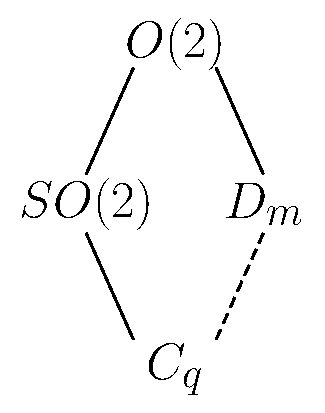
\includegraphics[height=0.15\textheight]{../figs/O2lattice}
~~~~(\textit{b})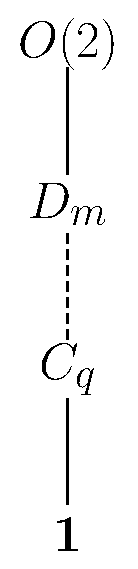
\includegraphics[height=0.15\textheight]{../figs/O2stablattice}
\end{center}
\caption[O(2) lattices]{
    {\small
    (a) \On{2} subgroup lattice, (b) \On{2} isotropy lattice for the action
	defined by \refeq{eq:O2stndrd}. In both figures dashed lines indicate
	containment only when $q$ divides $m$, while the relations $\Cn{q}\prec\Cn{m}$
	and $\Dn{q}\prec\Dn{m}$ when $q$ divides $m$ are not drawn. For the isotropy lattice $m,q\le n$.
	}}
\label{fig:O2lattice}
    \vspace*{-5pt}
\end{figure}
%%%%%%%%%%%%%%%%%%%%%%%%%%%%%%%%%%%%%%%%%%%%%%%%%%%%%%%%%%%%%%%%%

\end{example}

A general procedure exists\rf{gatermannHab} to determine which subgroups in the subgroup lattice of a group $\Gamma$ are isotropy
subgroups when $\Gamma$ acts faithfully on $\Rls{n}$.
For each subgroup $K$ (or more precisely for each subgroup class represented by $K$)
determine the dimension of the \fixedsp. Then we trace the subgroup lattice: For each subgroup
$K$ we compare $\dim(Fix(K))$ to $\dim(Fix(H))$ for every $H\subseteq\Gamma$ for which $K\subset H$.
If  $\dim(Fix(K))=\dim(Fix(H))$ then $K$ is not an isotropy subgroup. The determination of the dimension of the
\fixedsp\ of a subgroup $K$ can be done by means of the following trace formula if an explicit representation
$\rho(K)$ of $K$ is known or if one is able to determine the character of the representation by other means:
\beq
	\dim(Fix(K))=\frac{1}{|K|}\sum_{\kappa\in K} \trace(\rho(\kappa))\,.
\eeq


\subsection{Group action types}

In this section we state some definitions of different types of group actions.

\begin{definition}
\label{def:free}
\index{free}
A group $\Gamma$ acts freely on $\Manif$ if all isotropy subgroups are trivial: \stab{x}=\{e\} for all $x\in \Manif$.
$\Gamma$ acts locally freely if all isotropy subgroups are discrete subgroups of $\Gamma$.
\end{definition}

\begin{example}
The action \refeq{eq:SO2act} of \SOn{2} on \Rls{5} is not free (or even locally free), while the same action on $\Manif^*$ is free. If we don't
restrict $\theta$ in $[0,2\pi)$ then the group $\Rg{}$ acts locally freely on $\Manif^*$
since the isotropy subgroup is the discrete subgroup $2\pi\mathbb{Z}$ of integer multiples of $2\pi$.
\end{example}

\begin{example}
The action \refeq{eq:O2stndrd} of \On{2} is locally free on $\Clx{n}\setminus\{0\}$ but not on \Clx{n}.
\end{example}

\begin{definition}
\label{def:faithfull}
\index{faithful}
A group $\Gamma$ acts faithfully (or effectively) on $\Manif$ if and only if $\bigcup_{x\in\Manif}\stab{x}={e}$.
\end{definition}

An immediate consequence of \refLem{lem:NlzActs}
is that $\Nlz{\Sigma}/\Sigma$ acts faithfully on \Fix{\Sigma}.


\begin{example}
 The actions \refeq{eq:SO2act} of \SOn{2} and \refeq{eq:O2stndrd} of \On{2} are faithful.
\end{example}

\begin{definition}
\label{def:regular}
\index{regular}\index{semi-regular}
A group $\Gamma$ acts semi-regularly on $\Manif$ if all its orbits have the same dimension.
If in addition for each point $x\in \Manif$
there exists an arbitrarily small neighborhood $U$ such that each orbit of $\Gamma$ intersects $U$ in a pathwise connected subset, then the group
acts regularly.
\end{definition}
\ES{Think of regular versus semi-regular action as the group orbit being circle versus a spiral. I'll try to find a specific example of semiregular action.}
\ES{We can write in summary: free $\Rightarrow$ locally free $\Rightarrow$  semi-regular.}

\begin{example}
 Action \refeq{eq:SO2act} of $\SOn{2}$ is regular on $\Manif^*$ but not on $\Rls{5}$.
\end{example}


\begin{example}
Since the action \refeq{eq:O2stndrd} of \On{2} on $\Clx{n}\setminus\{0\}$ is free it is also semi-regular. Indeed, from \refPro{pro:dimOrb} all group orbits of points $x\in\Clx{n}\setminus\{0\}$ are $1$-dimensional.
\ES{This will turn out to be important when applying moving frame method.}.
\end{example}

The group orbits of an effective and regular or semi-regular action of a Lie group $\Gamma$ on a manifold \Manif\ form a foliation of \Manif\ES{Is this related to us being able to construct a local cross-section?}.

\PublicPrivate{}{
\subsection{Principal fibre bundles}

Assume a Lie group $\Gamma$ acts\ES{Any restriction on how it acts? In definition in Isham the term G-space is used, which I don't understand since he doesn't define it.} on a topological space $\tSp$. We call the bundle $(\tSp,\prj,\bSp)$ a \emph{$\Gamma$-bundle} if it is isomorphic to $(\tSp,\rho,\tSp/\Gamma)$. The fibres over the points of the base space $\tSp/\Gamma$ are the group orbits of points in $\tSp$.
Thus in general \ES{Can we
substitute ``in general'' with ``if $\Gamma$ does not act freely on $E$ then''} the bundle $E$ is not a fibre bundle since the fibres are not homeomorphic to each other. If $\Gamma$ acts freely on
$\tSp$ then the $\Gamma$-bundle is a fibre bundle with fibre $\Gamma$ and is called a \emph{principal $\Gamma$-bundle}, while $\Gamma$ is called the structure group of the bundle.
}%end \PublicPrivate

\section{Symmetries of solutions}

In the preceding section we concentrated on symmetries of the space on which a group acts.
Solutions of a differential equation do not necessarily have the full symmetry group $\Gamma$ of the differential
equation.
    \ES{Rewrite or drop: Their symmetry group is the
isotropy subgroup of the invariant subspace they live in and
this is why one cares about isotropy subgroups. Thus the
stratification by orbit type can be used to characterize
solutions as well.} The discussion flows better if we start
from the simplest solutions, \eqva, and then consider more
complicated solutions.

\subsection{\Eqva}
\label{sec:equilSym}

% Equilibria satisfy,
% \beq
% 	\vf(x)=0\,.
% \eeq

An {\eqv} with full symmetry lies in $\Fix{\Gamma}$,  the
orbit type is $\Idg$ and thus the multiplicity of the solution
is one. Note that if $\dim\Fix{\Gamma}=0$, since \fixedsp s are
flow invariant, the solution has to be an {\eqv}.

An {\eqv} $x$ with isotropy subgroup
$\stab{x}\subsetneq\Gamma$ has less than full symmetry.
According to \refPro{pro:dimOrb} this {\eqv} with orbit
type $\Gamma/\stab{x}$ does not come alone. If $\Gamma$ is
finite there are  $|\Gamma|/|\stab{x}|$ \eqva\ in the group
orbit of $\Gamma$. If $\Gamma$ is continuous then there is a,
possibly disconnected, manifold of \eqva\ of dimension
$\dim \Gamma - \dim \stab{x}$ passing through $x$.

\subsection{Periodic orbits}
\label{sec:poSym}

Let $x_p$ be a periodic orbit of \refeq{eq:difeq} with period $T_p$. Then, by equivariance, $\gamma x_p$
is another periodic orbit, for any $\gamma\in\Gamma$. From uniqueness of solutions $x_p$ and $\gamma x_p$
are either identical or disjoined.

If they are identical we must have,
\beq
	\gamma x_p(t+\theta) = x_p(t)
\eeq
for some $\theta\in S^{1}=[0,T]$. In Golubitsky and Stewart\rf{golubitsky2002sp} $(\gamma,\theta)\in \Gamma \times S^1$ is called a \emph{spatio-temporal
symmetry} of the solution $x_p$. Spatio-temporal symmetries for which $\theta=0$ are called \emph{spatial}
symmetries. 
% Alternatively we might say that a spatial symmetry is in the global isotropy subgroup $\globstab{x_p(t)}$ of $x_p(t)$ while the spatial part of a spatio-temporal symmetry is in the isotropy subgroup $\stab{x_p(t)}$.
The term spatial and spatio-temporal should not be confused with the terms used in the context of PDEs, here
spatial refers to \statesp. See Golubitsky and Stewart\rf{golubitsky2002sp} for more details.

If the periodic solutions are disjoint their multiplicity (if $\Gamma$ is finite), or the dimension
of the manifold swept under the group action (if $\Gamma$ is continuous) can be determined by application
of \refPro{pro:dimOrb} for any periodic point.

\subsection{\Reqva}

Let $\Gamma$ be compact. A group orbit of a point $x$ that is flow invariant is called a \reqv.
That is, there is dynamics only in the direction of the group action and in a frame moving along the group orbit with velocity given by the right hand side of \refeq{eq:difeq} the \reqv\ appears as an \eqv. Alternatively
we may view a \reqv\ as a group invariant periodic orbit, satisfying
\beq
	x(t)=\gamma_t x_0
\eeq
for a curve $\gamma_t\in\Gamma$.

\Reqva\ are a hallmark of systems with continuous symmetry. Unless a discrete subgroup
enforces it, there is no reason we should expect not to have dynamics in the direction of
group action and we expect to have \reqva. For the connection of this statement
to the genericity of bifurcations with continuous symmetry see \refref{golubitsky2002sp}.

\subsection{Relative periodic orbits}

For $\Gamma$ compact, a \rpo\ is a trajectory satisfying the condition
\beq
	x(t+T)=\gamma x(t)\,,
	\label{eq:rpoDef}
\eeq	
for all $t$ and for some group element $\gamma\in\Gamma$ and period $T$. In \refref{Krupa90}, Krupa proves
that the closure of a \rpo\ is a torus and provides a bound for its dimension. Another way to view
{\rpo s} is as {\po s} of the reduced dynamics, see \refsect{sec:symRed} bellow. Therefore, unless there is
a reason that enforces $\vf(t)$ in \refeq{eq:difeq} to be orthogonal to the direction of the group action,
one expects to find {\rpo s} in systems with continuous symmetry for the same reasons one expects periodic
orbits in generic dynamical systems with discrete or no symmetry.


\PublicPrivate{
    }{ % switch \PublicPrivate{
At the other extreme let's define a generic trajectory (with respect to symmetry) to be one that has no
symmetry and thus lives in the principal stratum and has group-orbit type $\Gamma$. For finite groups there exists a family of $|\Gamma|$ (disconnected) copies of the solution. For compact groups there exists a manifold of solutions of dimension $\dim \Gamma$.
    } % end \PublicPrivate{


    \PublicPrivate{
    }{ % switch \PublicPrivate{




\subsection{Equivariant bifurcation theory}

    } % end \PublicPrivate{



\section{Symmetry reduction}
\label{sec:symRed}

The purpose of symmetry reduction in differential equations is to project the dynamics to a space
in which the symmetry group $G$ acts trivially. Such a space is called \emph{orbit space} because each
group orbit of a point in original space is mapped to a single point in orbit space, or \emph{quotient
space} because the symmetry has been ``divided out'' or simply \emph{reduced space}. If the original
space is a manifold $\Manif$ it is then customary to write the quotient space as $\Manif/\Gamma$.
The resulting dynamical system is called \emph{image} of the original.

The stratification of $\Manif$ induced by the group action is carried over to the quotient space with each disconnected set in a stratum mapped to the same manifold in quotient space.
Yet, a fundamental problem with symmetry reduction is that the orbit space is in general not a manifold.
Unless the action of the group is free, group orbits do not have the same dimension and different
strata are mapped to manifolds of different dimension. We will see this property of quotient space
manifest itself in different ways depending on the reduction method but always introducing some
singularity even though there is nothing singular about $\Manif$ or the flow of the dynamical system
on it.


\subsection{Hilbert basis approach}


The most common approach to symmetry reduction is through the use of a Hilbert basis of invariant
polynomials. One computes a (non-unique) basis of linearly independent polynomials, invariant under the action
of the symmetry group (\cf \refref{gatermannHab} for a discussion of methods) and either rewrites
the dynamics in this basis or maps the solutions to the polynomials.
We will describe how this approach works for the example of \CLe in \refsect{sec:CLe}.
The reader is referred to the book of Gilmore and
Lettelier\rf{GL-Gil07b} for a very detailed discussion of
symmetry reduction. For the action \refeq{eq:SO2act} of
$\SOn{2}$ on \Rls{5} a Hilbert basis\rf{GL-Gil07b}  is
\beq
\begin{split}
	u_1 &= x_1^2+x_2^2 \cont
	u_2 &= y_1^2+y_2^2 \cont
	u_3 &= x_1 y_2-x_2 y_1\cont
	u_4 &= x_1 y_1+x_2 y_2\cont
	u_5 &= z\,.
	\label{eq:ipLaser}
\end{split}
\eeq
The polynomials in a Hilbert basis are linearly independent, but functionally dependent through
relation called \emph{syzygies}. For polynomials \refeq{eq:ipLaser} the syzygy is
\beq
 	u_1u_2 -u_3^2-u_4^2 =0\,.
	\label{eq:syzLaser}
\eeq

When one takes syzygies into account in rewriting the dynamical
system, singularities are introduced. Moreover when one
\emph{lifts} the dynamics from the quotient space $\Manif/G$ to
the original space $\Manif$ the transformations have
singularities at the \fixedsp s of the isotropy subgroups in
$\Manif$, in the optima case, \cf \refref{GL-Gil07b}. Those
singularities do not seem to restrict our ability to use
invariant polynomials to obtain symmetry reduced projections of
the dynamics as we will see in \refchap{chap:lasers}.

What restricts the utility of Hilbert basis methods is that the
determination of a Hilbert basis becomes computationally
prohibitive as the dimension of the system or of the group
increases\rf{gatermannHab,ChossLaut00} and typically
computations are constraint to dimension smaller than ten. As
our goal is to quotient continuous symmetries of
high-dimensional flows, specifically those arising from
truncations of the \KS\ and Navier-Stokes flows
and thus we need an efficient framework.


\subsection{Moving frames}
\label{sec:mf}

In this section we present the method of moving frames
    \PC{do they really say ``moving coframes'' rather than ``comoving frames''? {\bf ES}: Yes, they really do. They refer to
Cartan's method as method of ``moving frames'' and they claim it to be a special (and less rigorous) case of the moving coframe method.
I don't know Cartan's method and the two papers of Fels and Olver\rf{FelsOlver98,FelsOlver99} are lengthy and technical. Olver's
book is readable but I it doesn't describe Cartan's method. I think they say ``moving'' rather than ``comoving" frames
because one only comoves in the direction of group action.}
of Cartan\rf{CartanMF} in the formulation of Fels and Olver\rf{FelsOlver98,FelsOlver99}, also \cf~\refref{OlverInv} for
a pedagogical exposition and the proofs of theorems listed here. Its purpose is to generate functionally
independent invariants for the action of a group $\Gamma$ on a manifold $\Manif$ under certain assumptions,
and is not restricted to reduction problems. \ES{Use elsewhere: Fundamental here
means that they can be used to generate all other invariants.}
\ES{The name ``moving coframes'' arises through the use of Maurer-Cartan form which is a coframe on the Lie group $\Gamma$, in the sense that they form a poinwise basis for the cotangent space.}
nec

In the following let $\Gamma$ be $r$-dimensional and act on a $n$-dimensional manifold $\Manif$.
\begin{definition}
 A moving frame is a smooth $\Gamma$-equivariant mapping $\rho:\,\Manif \rightarrow \Gamma$.
\end{definition}
One distinguishes between left moving frames for which the equivariance condition is $\rho(\gamma x)=\gamma\rho(x)\,,\ x\in\Manif\,,\ \gamma\in\Gamma$ and right moving frames for which the equivariance condition is $\rho(\gamma x)=\rho(x)\gamma^{-1}\,,\ x\in\Manif\,,\ \gamma\in\Gamma$.

The following existence theorem for moving frames will be very important.

\begin{theorem}
 A moving frame exists in a neighborhood of a point $x\in \Manif$ if and
 only if $\Gamma$ acts freely and regularly near x.
\end{theorem}


For groups acting regularly we can define a cross-section for the group orbits.


\begin{proposition}%[\rf{OlverInv}]
 \label{pro:crossExists}
\index{cross-section}
 Let $\Gamma$ act regularly on a $n$-dimensional manifold $\Manif$ with $r$-dimensional orbits.
 Define a (local) \emph{cross-section}
 to be an $(n-r)$-dimensional submanifold $K$ of $\Manif$ such that $K$ intersects each orbit transversally and at most once. If a Lie group $\Gamma$ acts regularly on a manifold $\Manif$, then one can construct a local cross-section passing through any point $x\in \Manif$.
\end{proposition}

\ES{Is this cross-section related to a cross-section in a $\Gamma$-bundle?
In other words, can we interpret
the latter as a submanifold in total space \tSp\ of a $\Gamma$-bundle $(\tSp,\pi,\tSp/\Gamma)$? }


\begin{theorem}
 Assume the conditions of \refPro{pro:crossExists} hold and let $K\subset\Manif$ be a cross-section.
 For $x\in \Manif$, let $g=\rho(x)$ be the unique group element that maps $x$ to the
 cross-section: $g z = \rho(z) z\, \in K$. Then $\rho:\Manif\rightarrow G$ is a right moving frame.
\end{theorem}

A cross-section $K$ can be defined by means of level sets of functions $K_i(x)=c_i$,
where $x\in V$ and $i=1,\ldots,r$. If the $K_i(x)$
coincide with the local coordinates $x_i$ on the manifold $V$, \ie~$K_i(x)=x_i$,
then we call $K$ a \emph{coordinate cross section}.

\begin{example}
Consider the standart action of $\SOn{2}$ on \Rls{2}:
\beq
	(x,y) \mapsto (x\cos\theta -y \sin\theta,\,x\sin\theta +y \cos\theta )
\eeq
which is regular on $\Rls{2}\backslash\{0\}$. Thus we can define
a cross-section by, for instance, the
positive $y$ axis: $x=0,\,y>0$.
We can now construct a moving frame as follows. We write out
explicitly the group transformations:
\begin{subequations}
\begin{align}
 	\overline{x} &= x \cos\theta - y \sin\theta\label{eq:explSO2stnd1}\cont
	\overline{y} &= x \sin\theta + y \cos\theta\label{eq:explSO2stnd2}\,.
\end{align}
\end{subequations}
Then set $\overline{x}=0$ and solve \refeq{eq:explSO2stnd1} for the group
parameter to obtain the moving frame
\beq
	\theta=\tan^{-1}\frac{x}{y}
	\label{eq:SO2stndMF}
\eeq
which brings any point  back to the cross-section.\footnote{Implementation note: Here it is important that $\tan^{-1}$
distinguishes quadrants on the $(x,y)$ plane so that we get the correct geometric operation.} Substituting \refeq{eq:SO2stndMF} in the remaining equation. We get
the $\SOn{2}$-invariant expression
\beq
	\overline{y} = \sqrt{x^2+y^2}\,.
\eeq
\end{example}

The above \emph{normalization} procedure for the computation of
invariants applied in the example of $\SOn{2}$ can be applied
in much more general situations as follows. Assume $\Gamma$
acts (locally) freely\ES{The condition of free action can be
relaxed\rf{OlverInv}.} on \Manif\  and thus $\Gamma$-orbits
have the same dimension, say $r$, as $\Gamma$.  Choose a
coordinate cross-section $K=\{x_1=c_1,\ldots,x_r=c_r\}$ defined
by the first $r$ coordinates (relabel coordinates as
necessary). Introduce local coordinates $g=(g_1,\ldots,g_r)$ on
$\Gamma$ in the neighborhood of the identity.
The group transformations are
\beq
	\overline{x}= g \cdot x = w(g,x)\,.
	\label{eq:transNorm}
\eeq
Equating the first $r$ components of the function $w$ to the constants in the definition
of the cross-section $K_i(x)=c_i$ yields the \emph{normalization equations} for $K$:
\beq
	\overline{x}_1=w_1(g,x)=c_1,\ldots,\overline{x}_r=w_r(g,x)=c_r\,.
	\label{eq:normalization}
\eeq
From the definition of cross-section and the Implicit Function Theorem the normalization equations
\refeq{eq:normalization} can always be solved for the group parameters in terms of $x$,
yielding the moving frame associated with $K$: $g=\gamma(x)$. Substitution
of the moving frame equation back to \refeq{eq:transNorm} will yield the $n-r$
\emph{fundamental invariants}, in the sense that any other invariant can be expressed
as a function of $\overline{x}_2,\overline{y}_1, \overline{y}_2,\overline{z}$ and they are functionally independent.
Thus they serve to distinguish orbits in the neighborhood of the cross-section, \ie~two points lie on the same group
orbit if and only if all the fundamental invariants agree. For proof \cf~\refrefs{FelsOlver98,FelsOlver99}.

There exist two methods to convert a non-free\ES{but effective} action of a group $\Gamma$ on a
manifold $\Manif$ to a free action: one either prolongs the action to jet space and thus calculates
differential invariants, or considers the action of the group in $n$ copies of $\Manif$ with $n>>0$
and thus calculates joint invariants. The second method will not be helpful for us since the dimension
of the manifolds that we are interested in is already very high. We have not found a way to implement
the method of prolongation efficiently for the problems considered here. The way to get around of
non-free actions will be explained in \refsect{laserMFnum}.

\ES{It would appear removing a continuous symmetry is a simple task. Yet, the problem arises due to the structure of the group action. If we have isotropy subgroups and the action is not free then there are points
with less symmetry: the source of singularities.}
